\section{Detailed Design}
\subsection{Our design}
\subsubsection{Class diagram}

\begin{figure}[H]
 \centering
 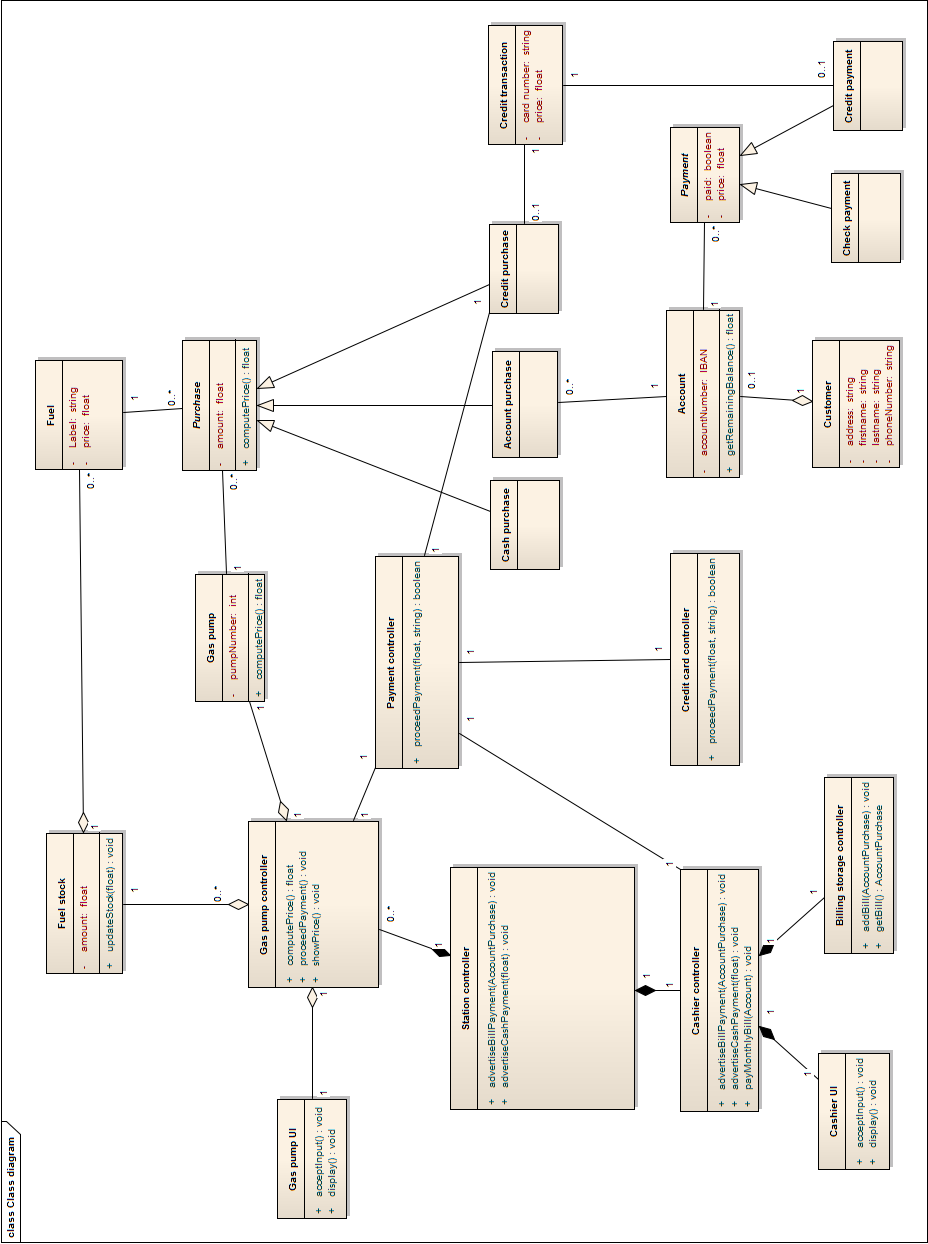
\includegraphics[width=\textwidth]{../ClassDiagram.png}
\end{figure}

\subsubsection{Description of classes}

\paragraph{Station controller}
The station controller is the main controller of the application. It has a list of Gas pump controller and a Cashier controller. 

\paragraph{Cashier controller}
It is responsible for managing all the interaction with the cashier. That's why it has a Cashier UI. It also has a Billing storage controller to be able to retrieve accounts and add bills when the user when to pay by monthly bill.

\paragraph{Cashier UI}
This class is the graphical interface presented to the cashier that allows him to input some payments or bills and display information.

\paragraph{Billing storage controller}
This controller manages the accounts that are stored in a database. So it contains a list of accounts.

\paragraph{Gas pump controller}
This controller is responsible for all the interactions with the customer and the fuel stock.
It contains a gas pump and is responsible for managing it. It has a Gas pump UI to interact with the customer. It also has a Fuel stock so that it can display the price.
At the end of the transaction, it is also responsible to proceed the payment. That's why it has a reference to a Payment controller.

\paragraph{Gas pump}
This class represents a real gas pump of the station. It has a method to compute the price of the last transaction that actually calls the same method from the Purchase class.
It has a list of references to some purchases that were made at that specific gas pump.

\paragraph{Gas pump UI}
This class is the graphical interface presented to the customer and is responsible for the interactions with the customer. It can display information and accept inputs that it will transmit the its controller.

\paragraph{Fuel stock}
This class represents the current stock available in the tank (amount attribute) of the station for a specific type of fuel. That's why it has a reference to Fuel.
Its only method is updateStock that receive a volume of fuel consumed or added to the stock and update the inventory database.

\paragraph{Fuel}
This class is a model representing a type of fuel with its price and label.

\paragraph{Purchase}
It is an abstract class representing a purchase made by a customer to a specific gas pump. It contains the amount of fuel taken at the pump and a reference to the fuel type so that it can compute the price of the transaction.

\paragraph{Cash purchase, Account purchase and Credit purchase}
Those three classes all extend the abstract class Purchase.
The cash purchase just represents a simple cash transaction, with no special attribute.
The account purchase is linked to an account and represent a purchase paid by monthly bill. 
A credit purchase is linked to a credit transaction and represent a purchase paid by credit card.

\paragraph{Payment controller}
This controller is responsible for doing a payment. It has access to the credit card controller and a credit purchase instance that represent the current payment to be done by credit card. Its only method is used by the Gas pump controller to proceed to the payment.

\paragraph{Credit card controller}
This controller is responsible for interacting with the external credit card reader and credit card system. 

\paragraph{Credit transaction}
This model class represents a transaction made by credit card. It has 3 fields: the card number, the price and the date of the transaction.

\paragraph{Account}
This model class represents the account of a customer. It has an account number and a list of payments. It can be used to compute its remaining balance, i.e. the amount that the customer must still pay. This is done by iterating over the payments list and adding the price of the unpaid payments.

\paragraph{Customer}
This model class represents a customer with all the needed fields.

\paragraph{Payment}
This abstract model class represents a payment linked to an account. Its state stored the price and a boolean that says if the payment has already been paid or not.

\paragraph{Check payment and Credit payment}
Those 2 classes extend the abstract Payment class and represent a concrete payment that is either done by check or credit card.


\subsubsection{Uses diagram}

\begin{figure}[H]
 \centering
 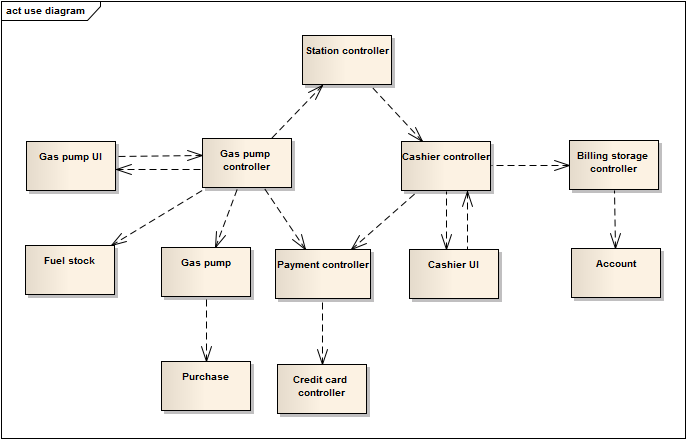
\includegraphics[width=\textwidth]{../useDiagram.png}
\end{figure}
There are 2 loops in this Uses diagram:
\begin{itemize}
	\item between \textit{Gas pump UI} and \textit{Gas pump controller}
	\item between \textit{Cashier UI} and \textit{Cashier controller}
\end{itemize}
But this is not really a problem because there are just between a view and its controller. It makes senses that the controller uses the view to update it and that the view uses the controller to notify it when an user's action occurs. We think that they can no be eliminated.


\subsection{Design Patterns}
The skeletons are written in Java.

\subsubsection{Template Method}
\begin{figure}[H]
 \centering
 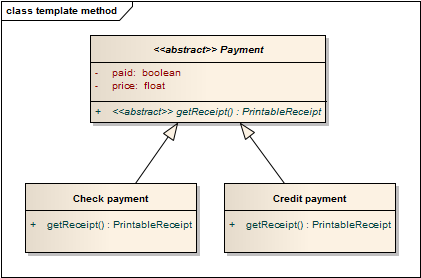
\includegraphics[width=0.75\textwidth]{../templateMethod.png}
\end{figure}

\lstinputlisting[language=java, inputencoding=utf8]{templateMethod.java}


\subsubsection{Strategy Pattern}
\begin{figure}[H]
 \centering
 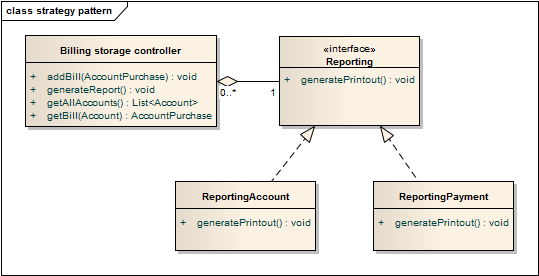
\includegraphics[width=0.8\textwidth]{../strategyPattern.png}
\end{figure}

\lstinputlisting[language=java, inputencoding=utf8]{strategyPattern.java}


\subsubsection{Decorator Pattern}
\begin{figure}[H]
 \centering
 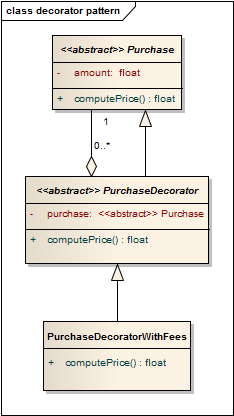
\includegraphics[width=0.35\textwidth]{../decoratorPattern.png}
\end{figure}

\lstinputlisting[language=java, inputencoding=utf8]{decoratorPattern.java}


\subsubsection{Observer Pattern}
\begin{figure}[H]
 \centering
 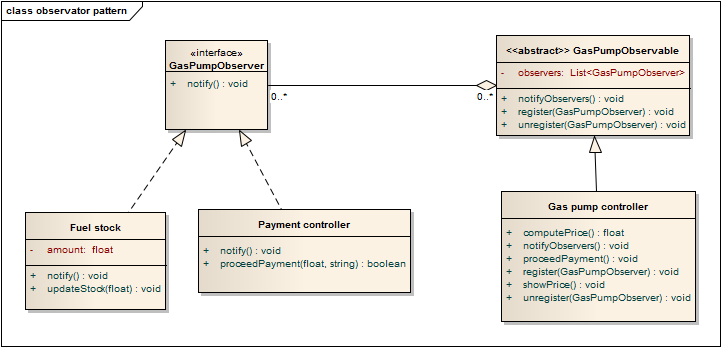
\includegraphics[width=0.9\textwidth]{../observatorPattern.png}
\end{figure}

\lstinputlisting[language=java, inputencoding=utf8]{observatorPattern.java}


\subsubsection{Composite Pattern}
\begin{figure}[H]
 \centering
 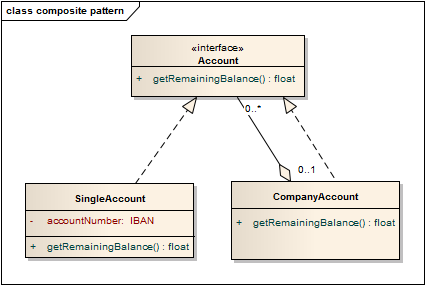
\includegraphics[width=0.8\textwidth]{../compositePattern.png}
\end{figure}

\lstinputlisting[language=java, inputencoding=utf8]{compositePattern.java}

We can see in the snippet of code above where the new methods are implemented.
But the existing methods (the getters and setters for the bank account in this case) are implemented in the SingleAccount class. If we had other pre-existing methods in the Account, they would be implemented in the new SingleAccount class and also in the CompanyAccount. To call those methods, the developer should have a reference to the concrete object, not the new Account interface (because it does not define other methods than \textit{getRemainingBalance()}.
